
\begin{savequote}[75mm]
%\begin{figure}[ht]
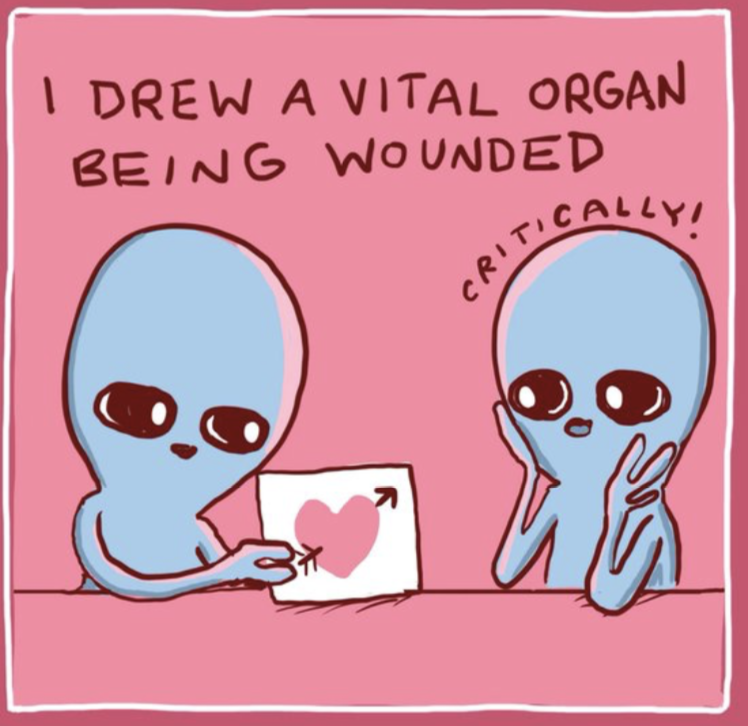
\includegraphics[width=0.75\linewidth]{./figures/graphical/comic.png}
%\label{sketch_gallery}
%\vspace{-1em}
%\end{figure}
\end{savequote}

\chapter{Graphical convention formation during visual communication}
\graphicspath{{./figures/graphical/}}

From ancient etchings on cave walls to modern digital displays, visual communication lies at the heart of key human innovations (e.g., cartography, data visualization) and forms a durable foundation for the cultural transmission of knowledge and higher-level reasoning.
Perhaps the most basic and versatile technique supporting visual communication is drawing, the earliest examples of which date to at least 40,000-60,000 years ago \cite{hoffmann2018u}.
What began as simple mark making has since been adapted to a wide array of applications, ranging from photorealistic rendering to schematic diagrams consisting entirely of symbols.

Even in the relatively straightforward case of drawing from life, there are countless ways to depict the same object.
How does a communication medium spanning such a broad range of appearances reliably convey meaning?
On the one hand, prior work has found that semantic information in a figurative drawing, i.e., the object it represents, can be derived purely from its visual properties \cite{FanCommon2018}.
On the other hand, other work has emphasized the role of socially-mediated information for making appropriate inferences about what even a figurative drawing represents \cite{goodman1976languages}.

\begin{figure}
\begin{center}
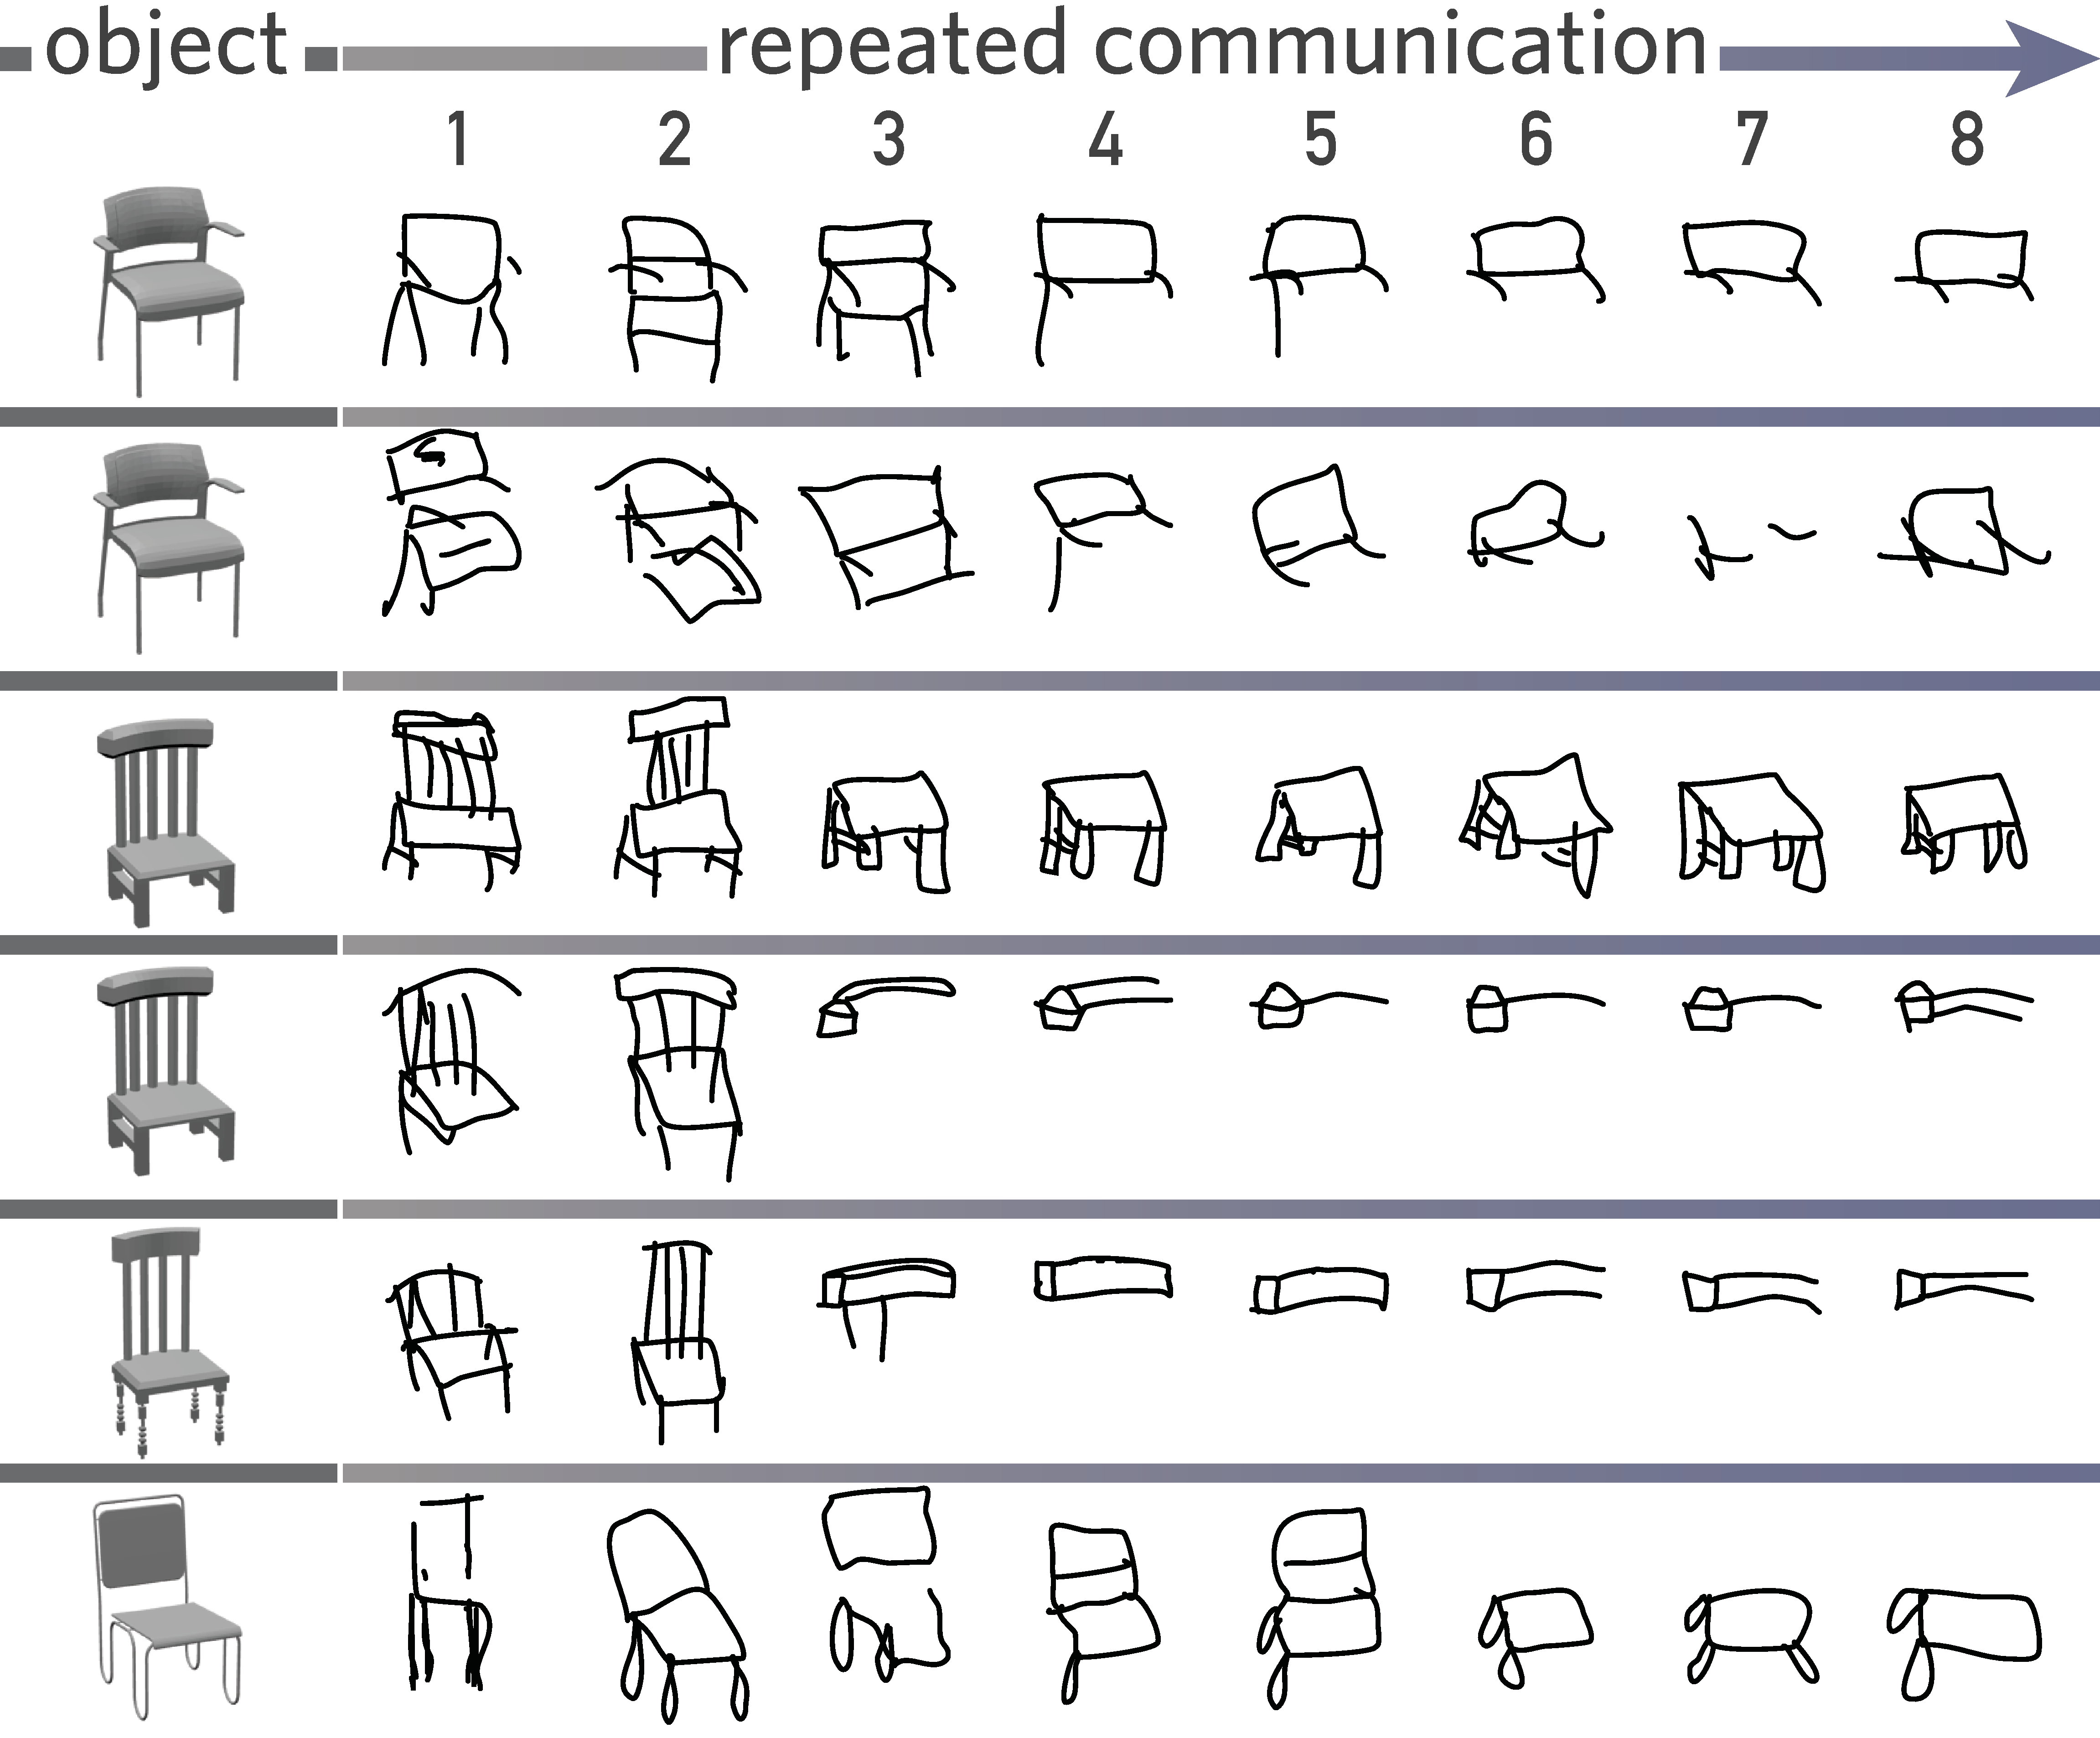
\includegraphics[width=0.7\linewidth]{sketch_gallery.pdf}
\caption{Repeated visual communication depicting the same object.}
\label{sketch_gallery}
\end{center}
\vspace{-1em}
\end{figure}

How can these two perspectives be reconciled?
Our approach is to consider the joint contributions of visual information and social context in determining how drawings derive meaning \cite{abell2009canny}, and to propose that a critical factor affecting the balance between the two may be the amount of shared knowledge between communicators.
Specifically, we explore the hypothesis that accumulation of shared knowledge via extended visual communication may promote the development of increasingly schematic yet effective ways of depicting an object, even as these \textit{ad hoc} graphical conventions may be less readily apprehended by others who lack this shared knowledge.

To investigate this hypothesis, we used an interactive drawing-based reference game in which two participants repeatedly communicated about visual objects.
We examined both how their task performance and the drawings they produced changed over time (see Fig.~\ref{sketch_gallery}).
Our approach was inspired by a large literature that has explored how extended interaction influences communicative behavior in several modalities, including language \cite{ClarkWilkesGibbs86_ReferringCollaborative,HawkinsFrankGoodman17_ConventionFormation}, gesture \cite{goldin1996silence}, and drawings \cite{garrod_foundations_2007,Galantucci:2005uh}.
There are three aspects of the current work that advance our prior understanding: \emph{first}, we include a control set of objects that were not repeatedly drawn but only shown at the beginning and end of the interaction, allowing us to measure the specific contribution of repeated reference vs. general practice effects; \emph{second}, we measure how strongly the visual properties of drawings drive recognition in the absence of interaction history for naive viewers, while equating other task variables; and \emph{third}, we employ recent advances in computer vision to quantitatively characterize changes in the high-level visual properties of drawings across repetitions.



%% galantucci2005experimental, fay2014creating, krauss1964changes, fay2010interactive

%% Figure 1 around here: (A) Stimuli. (B) Task (Sketcher/Viewer interface)
\begin{figure*}
\begin{center}
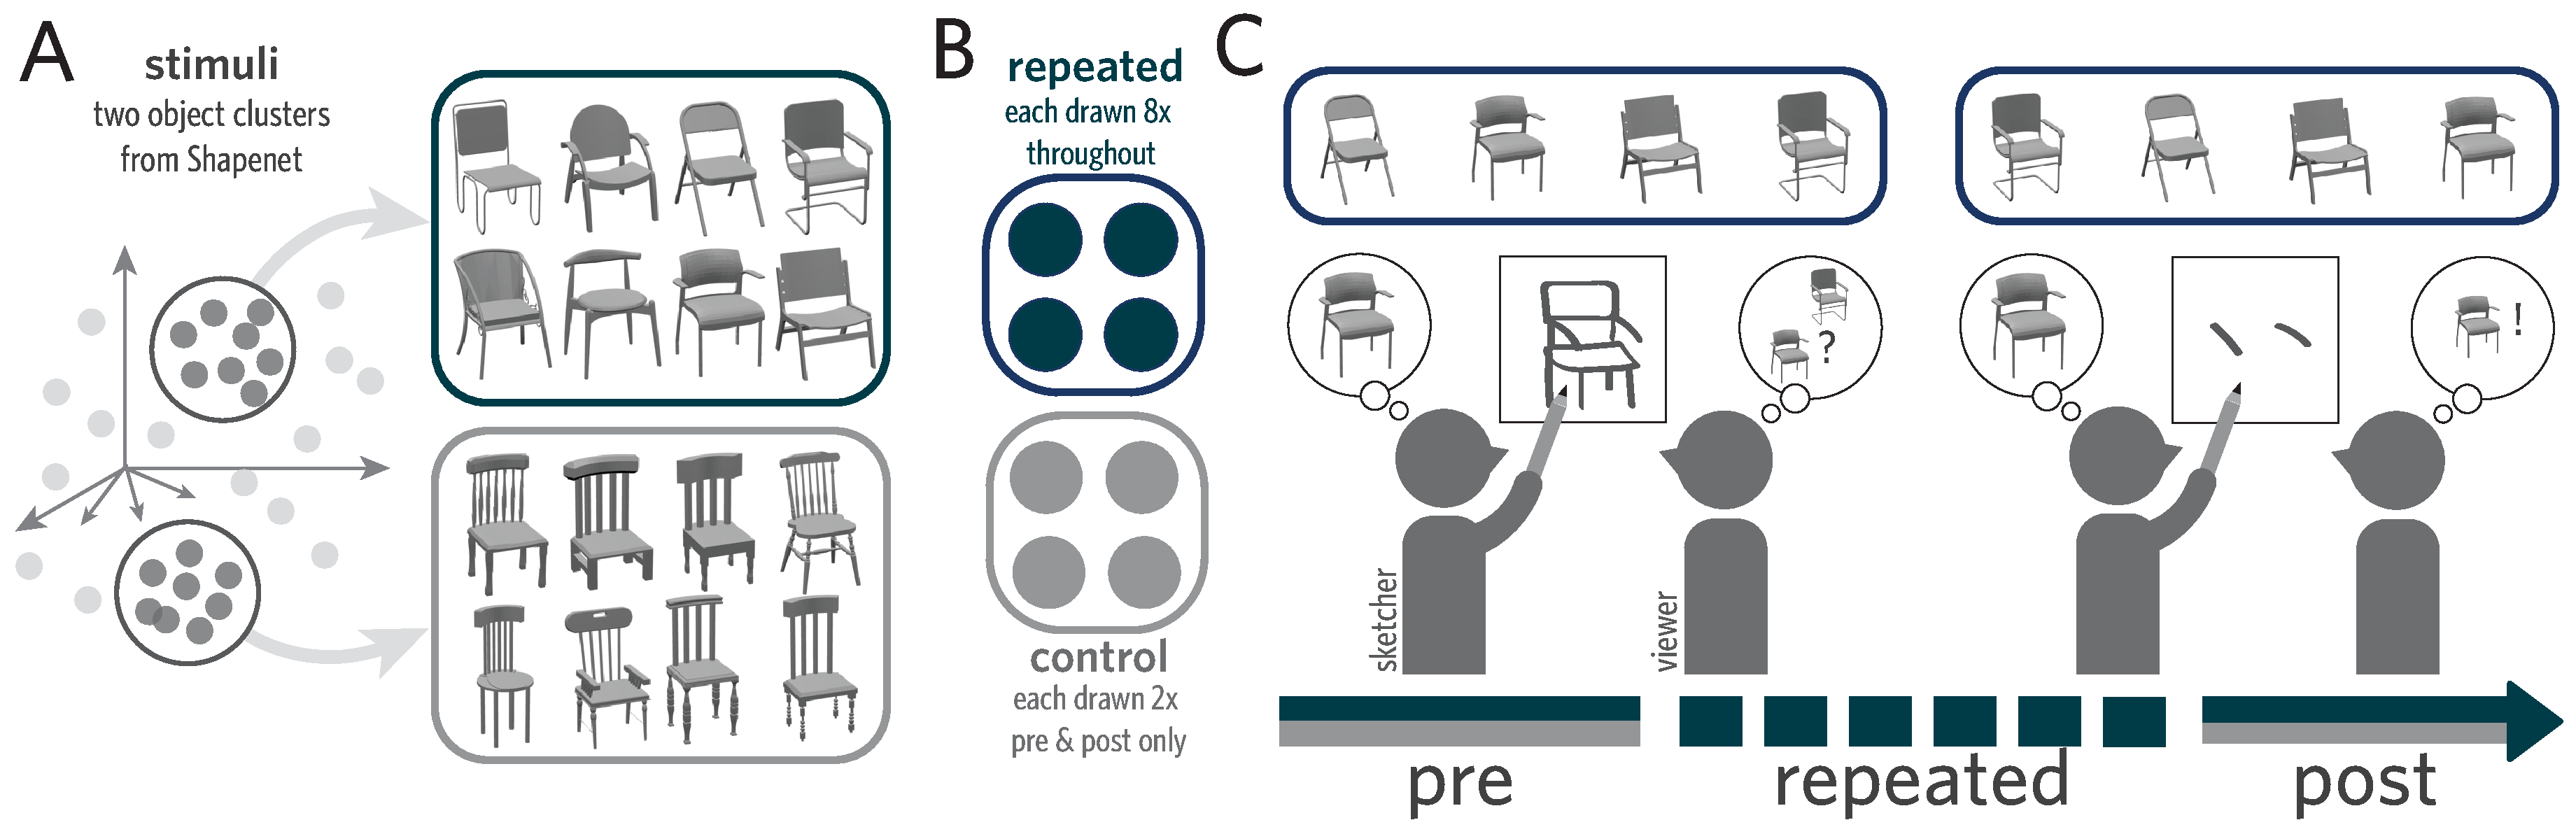
\includegraphics[width=0.95\linewidth]{task_stimuli.pdf}
\caption{(A) Stimuli from ShapeNet. (B) Each pair of participants was randomly assigned two sets of four objects, each set from one of the two categories. (C) Repeated objects drawn eight times throughout; control objects drawn once at the beginning and end of each interaction.}
\label{task_stimuli}
\vspace{-1em}
\end{center}
\end{figure*}

% extra: Galantucci:2005uh,healey2007graphical,theisen2010systematicity


\section{How does repeated reference support successful visual communication?}

%% intro to this section
Our first goal was to understand how people learn to communicate about visual objects across repeated visual communication.
To accomplish this, we developed a drawing-based reference game for two participants.
On each trial, both participants shared a \textit{communicative context}, represented by an array of four objects.
One of these objects was privately designated the `target' to the sketcher.
The sketcher's goal was to draw the target so that the viewer could select it from the array as quickly and accurately as possible.
We hypothesized that learning would be \emph{object-specific}: that over repeated visual reference to a particular object, participants would discover ways of depicting that object more effectively relative to non-repeated control objects.

%% methods
\subsection{Methods: Visual communication experiment}

\subsubsection{Participants} We recruited 138 participants from Amazon Mechanical Turk, who were grouped into 69 pairs \cite{Hawkins15_RealTimeWebExperiments}.
Within each experimental session, one participant was assigned the sketcher role and the other the viewer role, and these role assignments remained the same throughout the experiment.
%They were provided a base compensation of \$1.50 for participation and up to \$1.60 in bonus for high task performance.
Data from two pairs were excluded due to unusually low performance (i.e., accuracy $<$ 3 s.d. below the mean). In this and subsequent experiments, participants provided informed consent in accordance with the Stanford IRB.

\subsubsection{Stimuli}
%% provide justification for why we're using sets of similar objects
%% provide justification for why we're using images of real-world objects

In order to make our task sufficiently challenging, we sought to construct communicative contexts consisting of objects whose members were both geometrically complex and visually similar.
To accomplish this, we sampled objects from the ShapeNet \cite{chang2015shapenet}, a database containing a large number of 3D mesh models of real-world objects. % belonging to 55 different object classes.
We restricted our search to 3096 objects belonging to the \texttt{chair} class, which is among the most diverse and abundant in ShapeNet.
To identify groups of visually similar chairs, we first extracted high-level visual features from 2D renderings of each object using a deep convolutional neural network (DCNN) architecture, VGG-19 \cite{simonyan2014very}.
This network had been previously trained to recognize objects in photos from the ImageNet database \cite{deng2009imagenet}, containing 1.2 million natural photographs of 1000 different object classes.
Trained DCNN models have been shown to predict human perceptual similarity judgments about objects \cite{kubilius2016deep,peterson2018evaluating}, as well as neural population responses in visual cortex during object recognition \cite{yamins2014performance,gucclu2015deep}.
As such, they provide a principled choice of encoding model for extracting high-level visual information from images.
Following previous work that has employed DCNN models to evaluate perceptual similarity \cite{peterson2018evaluating,kubilius2016deep}, for each image we extract a 4096-dimensional feature vector reflecting activations in the second fully-connected layer (i.e., \texttt{fc6}) of VGG-19, a higher layer in the network.
We then applied dimensionality reduction (PCA) and $k$-means clustering on these feature vectors, yielding 70 clusters containing between 2 and 80 objects each.
Among clusters that contained at least eight objects, we manually identified two visual categories containing eight objects each (Fig.~\ref{task_stimuli}A).

\subsubsection{Task Procedure}

%% Trial-level event structure
% Drawings were collected in the context of an online, sketching-based reference game using the framework described in \citeA{Hawkins15_RealTimeWebExperiments}.
% The game involved two players: a \textit{sketcher} who aims to help a \textit{viewer} pick out a target object from a set of distractor objects by representing it in a sketch.
On each trial, both participants were shown the same set of four objects in randomized locations.
One of the four objects was highlighted on the sketcher's screen to designate it as the target.
%% Trial-level objective of sketcher and viewer
Sketchers drew using their mouse cursor in black ink on a digital canvas embedded in their web browser ($300 \times 300$ pixels; pen width = 5px).
Each stroke was rendered on the viewer's screen in real time and sketchers could not delete previous strokes.
The viewer aimed to click one of the four objects as soon as they were confident of the identity of the target, and participants received immediate feedback: the sketcher learned when and which object the viewer had clicked, and the viewer learned the true identity of the target.
Both participants were incentivized to perform both quickly and accurately.
They both earned an accuracy bonus for each correct response, and the sketcher was required to complete their drawings in 30 seconds or less.
If the viewer responded correctly within this time limit, participants also received a speed bonus inversely proportional to the time taken until the response.
%Otherwise, the viewer had no other means of communicating with the sketcher.

%% Two conditions: repeated and control

% Each pair of participants was randomly assigned two of these categories, and only the 16 objects from these two categories appeared as drawing targets during their session.

\subsubsection{Design}
For each pair of participants, two sets of four objects were randomly sampled to serve as communication contexts: one was designated the \emph{repeated} set while the other served as the \emph{control} set (Fig.~\ref{task_stimuli}B).\footnote{In half of the pairs, the four control objects were from the same stimulus cluster as repeated objects; in the other half, they were from different clusters. The rationale for this was to support investigation of between-cluster generalization in future analyses. In current analyses, we collapse across these groups.} % (N=34 for same; N=33 for different)
% These control objects were thus maximally perceptually similar to the repeated objects but were not repeatedly drawn and provided a tight baseline for object-specific effects.
%In the other half of pairs (N=XX pairs), the repeated set contained four randomly sampled objects from one category and the control set contained four randomly sampled objects from the other category.
The experiment consisted of three phases (Fig.~\ref{task_stimuli}C).
During the repeated reference phase, there were six repetition blocks of four trials, and each of the four \emph{repeated} objects appeared as the target once in each repetition block.
In a pretest phase at the beginning of the experiment and a posttest phase at the end, both repeated and control objects appeared once as targets (in their respective contexts) in a randomly interleaved order.
%Within this phase were six repetition cycles wherein each repeated object served as the target exactly once, and object order was randomized across repetition cycles.
% These control objects still shared many perceptual features with the repeated objects, but provided a measure of the more generic effects of task practice.

\begin{figure}
\begin{center}
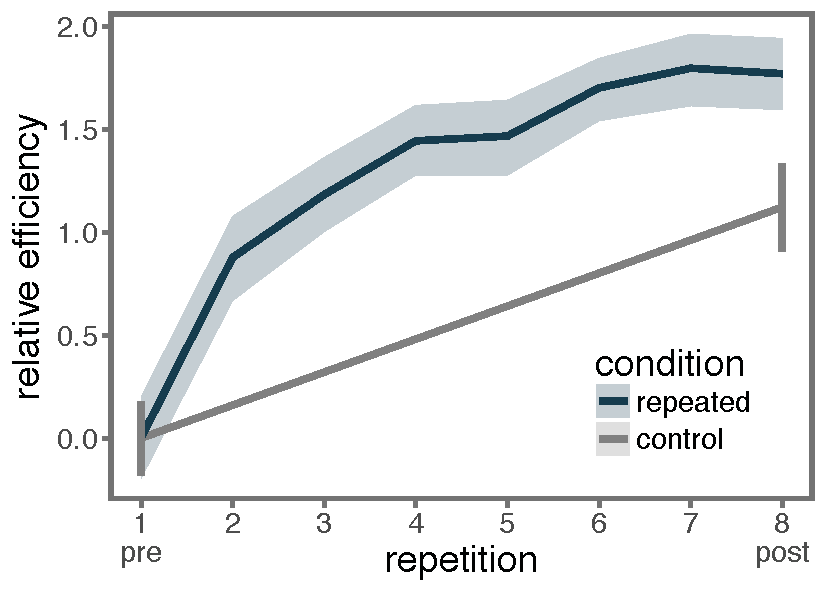
\includegraphics[width=0.88\linewidth]{refgame_BIS_timeseries.pdf}
\caption{Communication efficiency across repetitions. Efficiency combines both speed and accuracy, and is plotted relative to the first repetition. Error ribbons represent 95\% CI.}
\label{refgame_bis}
\end{center}
\end{figure}

\subsection{Results}

Because objects were randomly assigned to repeated and control conditions, we expected no differences in task performance in the pretest phase.
We found that pairs identified the target at rates well above chance in this phase (75.7\% repeated, 76.1\% control, chance = 25\%), suggesting that they were engaged with the task but not at ceiling performance.
% n  empirical_stat      ci_lower            mean               ci_upper
%67	-0.003731343	-0.07089552	-0.001317164	0.07089552
We found no difference in accuracy across conditions (mean difference: 0.3\%, bootstrapped CI: $[-7\%, 7\%]$).

In order to measure how well pairs learned to communicate throughout the rest of their interaction, we used a measure of communicative efficiency \cite<the \emph{balanced integration score,}>{Liesefeld2018} that takes both accuracy (i.e., proportion of correct viewer responses) and response time (i.e., latency before viewer response) into account.
This efficiency score is computed by first $z$-scoring accuracy and response time across repetitions within an interaction to map values from different interactions to the same scale, and then subtracting the standardized response time from standardized accuracy.
It is highest when pairs are both fast and accurate, and lowest when they make more errors and take longer, relative to their own performance on other trials.%\footnote{Results are similar for accuracy alone, but we adopted this integrated measure to better control for speed-accuracy tradeoffs.}

% Formula: bis_score ~ phase * condition + (1 + phase * condition | gameID)
%    Data: input
% Fixed effects:
%                    Estimate Std. Error        df t value Pr(>|t|)
% (Intercept)        -0.42302    0.05473 125.82978  -7.730 2.97e-12 ***
% phase1             -1.44656    0.10112 137.22562 -14.306  < 2e-16 ***
% condition1          0.35670    0.14118  70.83601   2.527  0.01376 *
% phase1:condition1  -0.64821    0.20974  94.62722  -3.091  0.00262 **
% ---
% Signif. codes:  0 ‘***’ 0.001 ‘**’ 0.01 ‘*’ 0.05 ‘.’ 0.1 ‘ ’ 1

To evaluate changes in communicative efficiency, we fit a linear mixed-effects model including random intercepts, slopes, and interactions for each pair of participants.
We found a main effect of increasing communicative efficiency for all targets between the \textit{pre} and \textit{post} phases ($b = 1.45,~t = 14.3,~p <0.001$), reflecting general improvements due to task practice.
Critically, however, this analysis also revealed a reliable interaction between phase and condition: communicative efficiency improved to a greater extent for repeated objects than control objects ($b = 0.648, ~t = 3.09,~p = 0.003$; see Fig.~\ref{refgame_bis}).
Analysis of changes in raw accuracy yielded a similar result: performance on repeated objects improved by 14.5\%, while performance on control objects only improved by 7.1\%.
Together, these data show that there are benefits of repeatedly communicating about an object that accrue specifically to that object, suggesting the formation of object-specific graphical conventions.
%\ndg{optionally: add the observation that the object-general boost seems to be achieved after the first trial, and is likely very general orientation to the task?}

% the benefits of repeatedly communicating about an object accrue more strongly to that object
% show gains in communicative efficiency are to some extent specific to the objects that were repeatedly referenced

% Optional: We found a similar pattern of results when we used the number of strokes in each drawing instead of drawing time in our estimate of communicative efficiency.

% Thus, participants converged on simpler, faster, and more communicatively successful graphical conventions for repeated objects, which only partially transferred to other objects.

%We clearly see that while the cost of sketching decreases, the accuracy of the viewer's guess of which object the drawing is referring to increases, suggesting that this reduction is meaningful.

%% task-level and object-level benefits of extended communication.

%Successful communication was primarily quantified as the viewer's accuracy in identifying the target.
%The investment of time was measured as the length of time between the beginning of the first stroke to the completion of the final stroke in each sketch, and the investment of ink was measured in two ways: as the number of strokes used for each drawing and the proportion of the drawing canvas filled by ink.

%This ensures that the reduction in the drawing duration and number of strokes over time is not due to the players losing interest or becoming less motivated during the game.

\section{What explains gains in efficiency?}

Our visual communication experiment established that pairs of participants coordinate on more efficient and \emph{object-specific} ways of depicting targets. % more efficiently across repetitions.
This raises the question: to what extent do these gains in efficiency reflect the accumulation of \emph{interaction-specific} shared knowledge between a sketcher and viewer, as opposed to the combination of task practice and the inherent visual properties of their drawings?

To disentangle the contributions of these different factors, we conducted two control experiments to estimate the how recognizable these drawings were to naive viewers outside the social context in which they were produced.
%Naive participants performed a drawing recognition task that closely matched the task of the viewer in
%In these experiments, we manipulated the sequence of drawings shown to naive participants in a recognition task.
Participants in one control group were shown a sequence of drawings taken from a single interaction, closely matching the experience of viewers in the communication experiment.
Participants in a second control group were instead shown a sequence of drawings pieced together from many different interactions, thus disrupting the continuity experienced by viewers paired with a single sketcher.
Insofar as interaction-specific shared knowledge contributed to the efficiency gains observed previously, we hypothesized that the second group would not improve as much over the course of the experimental session as the first group would.

%We manipulated the sequence of drawings participants saw such that
% with drawings produced in the earlier experiment.% and asked them to that closely matched the viewer's task in the earlier experiment, except here they knew their responses were not being provided as real-time feedback to the sketcher. %they were presented with drawings and guessed which of the four objects it referred to.
%\ndg{there's something missing on this motivation... maybe a hypothesis like "we expect viewer who see the same sequence of referential drawings to do as well, but viewers who see different ones not to? err...}
% , and they made their decision based on the final drawing, rather than being able to interrupt await additional information.

\subsection{Methods: Recognition Control Experiments}

\subsubsection{Participants}

We recruited 245 participants via Amazon Mechanical Turk.
We excluded data from 22 participants who did not meet our inclusion criterion for accurate and consistent response on attention-check trials (see below).

\begin{figure}[ht]
\begin{center}
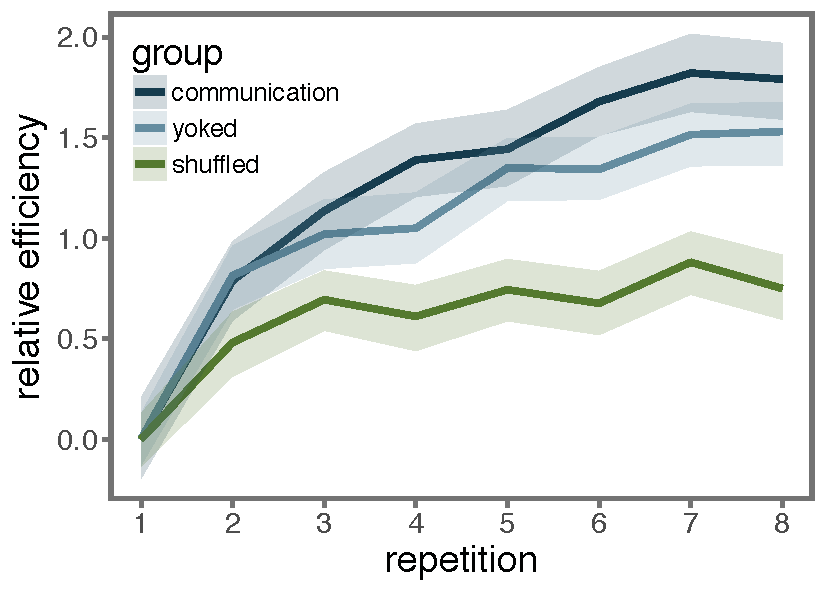
\includegraphics[width=0.88 \linewidth]{recog_BIS_timeseries.pdf}
\caption{Comparing drawing recognition performance between viewers in communication experiment with those of yoked and shuffled control groups. Error ribbons represent 95\% CI.}
\label{recog_bis}
\end{center}
\end{figure}


\subsubsection{Task, Design, \& Procedure}
%How does efficiency of graphical communication, measured by how accurately and quickly the viewer can select the target intended by the sketcher, change when we change the degree of interaction specificity?
%Here, we define interaction specificity based on both temporal structure (path dependence) and partner specificity.
%Therefore, we design several experiments that measure the recognizability of drawings and reaction times produced in the drawing task by third-party observers.

On each trial, participants were presented with a drawing and the same set of four objects that accompanied that drawing in the original visual communication experiment.
They also received the same accuracy and speed bonuses as viewers in the communication experiment.
%Their task was thus the same as the viewer's in the communication experiment, except they knew their responses were not being provided as real-time feedback to the sketcher.
To ensure task engagement, we included five identical attention-check trials that appeared once every eight trials.
Each attention-check trial presented the same set of objects and drawing, which we identified during piloting as the most consistently and accurately recognized by naive participants.
Only participants who responded correctly on at least four out of five of these trials were retained in subsequent analyses.

Each participant was randomly assigned to one of two conditions: a \textit{yoked} group and a \textit{shuffled} group.
Each yoked participant was matched with a single interaction from the original cohort and viewed 40 drawings in the same sequence the original viewer had.
Those in the shuffled group were matched with a random sample of 10 distinct interactions from the original cohort and viewed four drawings from each in turn, which appeared within the same repetition block as they had originally.
For example, if a drawing was produced in the fifth repetition block in the original experiment, then it also appeared in the fifth block for shuffled participants.

At the trial level, groups in both conditions thus received exactly the same visual information and performed the task under the same incentives to respond quickly and accurately.
At the repetition level, both groups received exactly the same amount of practice recognizing drawings.
Thus any differences between these groups are attributable to whether drawings came from the same communicative interaction, which would support the accumulation of interaction-specific experience, or from several different interactions, where such accumulation would be minimal.

\begin{figure*}
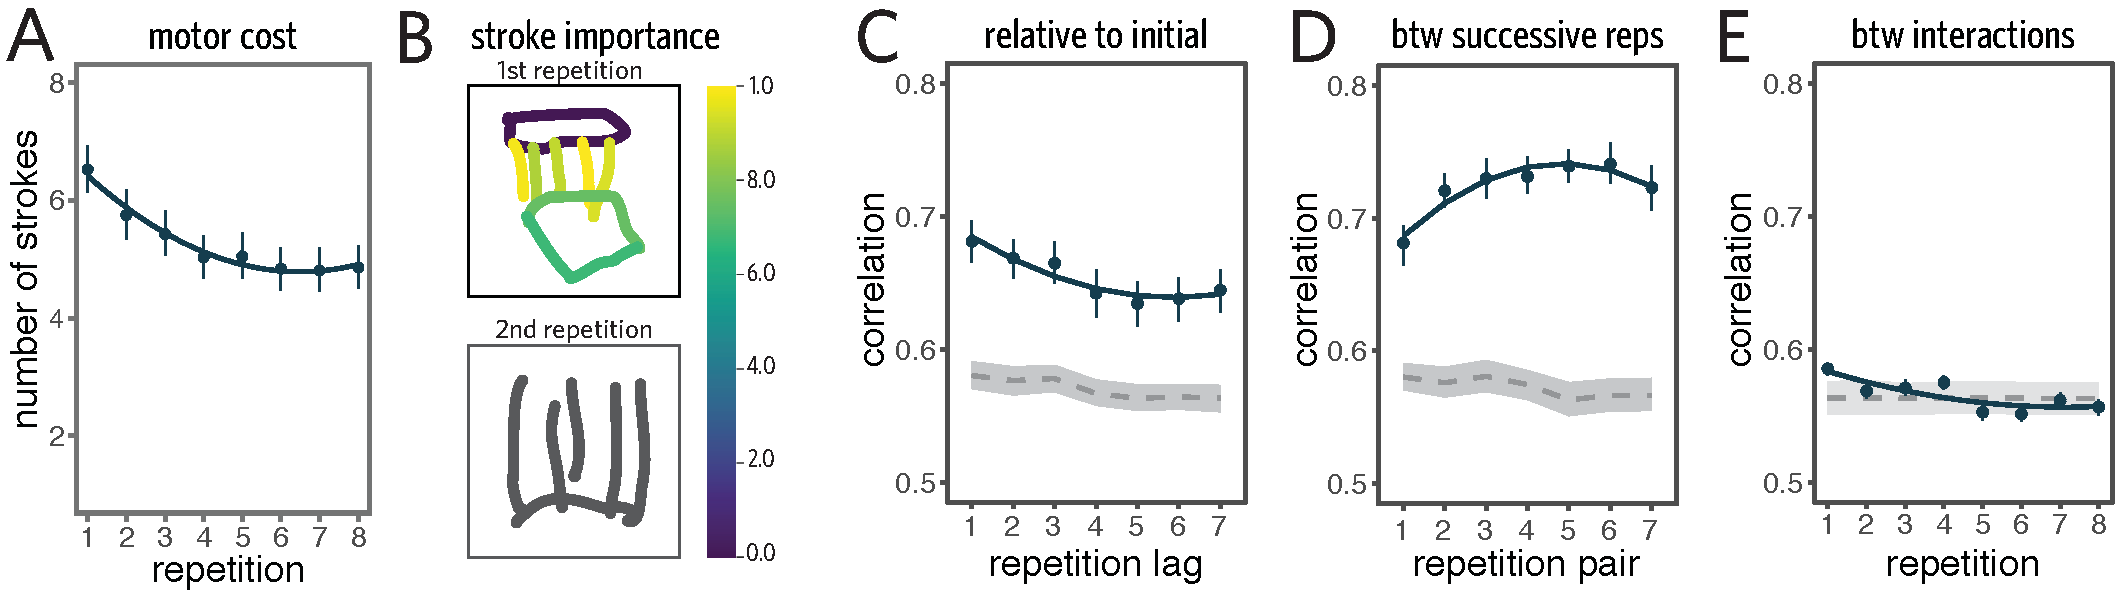
\includegraphics[width=0.92\linewidth]{drawing_changes.pdf}
\centering
\caption{(A) Sketchers use fewer strokes over time. (B) Visualizing importance of individual strokes in successive drawings. (C) Drawings become increasingly dissimilar from initial drawing. (D) Drawings become more consistent from repetition to repetition. %, becoming more internally consistent.
(E) The same object is drawn increasingly dissimilarly by different sketchers. %, suggesting multiple viable graphical conventions.
Error ribbons represent 95\% CI, dotted lines represent permuted baseline.}
\label{within-across}
\end{figure*}


\subsection{Results}

\subsubsection{Interaction-specific history enhances recognition by third-party observers}

% Linear mixed model fit by REML. t-tests use Satterthwaite's method ['lmerModLmerTest']
% Formula: bis_relative ~ version * repetition + (1 + repetition | gameID)
%    Data: d.recog %>% filter(version %in% c("yoked", "shuffled"))

% Fixed effects:
%                             Estimate Std. Error        df t value Pr(>|t|)
% (Intercept)                  0.43214    0.06485 287.50472   6.663 1.36e-10 ***
% versionshuffled             -0.13284    0.08954 287.50472  -1.484    0.139
% repetition                   0.18430    0.01440 326.27439  12.801  < 2e-16 ***
% versionshuffled:repetition  -0.09715    0.01988 326.27439  -4.888 1.60e-06 ***
% ---
% Signif. codes:  0 ‘***’ 0.001 ‘**’ 0.01 ‘*’ 0.05 ‘.’ 0.1 ‘ ’ 1

We compared the yoked and shuffled groups by measuring changes in recognition performance across successive repetitions using the same efficiency metric we previously used.
We estimated the magnitude of these changes by fitting a linear mixed-effects model that included group (yoked vs. shuffled), repetition number (i.e., first through eighth), and their interaction, as well as random intercepts and slopes for each participant.
While we found a significant increase in recognition performance across both groups ($b = 0.18, ~t = 12.8, ~p < 0.001$), %possibly reflecting general practice effects or inherent visual correspondences between drawings and the target object,  %10^{-15}$
%\ndg{the regression reported doesn't show the latter ("inherent...") since it's about difference over trials?}
we also found a large and reliable interaction:
yoked participants improved to a substantially greater degree than shuffled participants ($b = 0.10, ~t = 4.9, ~p<0.001$; Fig.~4).
Examining accuracy alone yielded similar results: the yoked group improved to a greater degree across the session (yoked: +15.8\%, shuffled: +5.6\%).
% was more accurate overall at identifying the target object (yoked: 75\%, shuffled: 69\%, $~t = 3.6, ~p < 0.001$)
Taken together, these results suggest that third-party observers in the yoked condition who viewed drawings from a single interaction were able to take advantage of this continuity to more accurately identify what successive drawings represented.
While observers in the shuffled condition still improved over time, being deprived of this interaction continuity made it relatively more difficult to interpret later drawings.

% in their ability to understand drawings even as the temporal order of the drawing was preserved.

%% ACCURACY LMER
% Formula: accuracy ~ version + (1 | gameID)
% Fixed effects:
% Fixed effects:
%                  Estimate Std. Error        df t value Pr(>|t|)
% (Intercept)       0.74912    0.01228 221.00001  60.982  < 2e-16 ***
% versionshuffled  -0.06081    0.01696 221.00001  -3.586 0.000413 ***
% ---

%% ACCURACY MEANS
% communication	0.8745336
% yoked	0.7491156
% shuffled	0.6883013

% We found that communicative efficiency increased overall between the \textit{pre} and \textit{post} phases ($b = 1.45,~t = 14.3,~p <0.001$), reflecting generalized improvements as a consequence of extended interaction.
% Critically, this analysis also revealed a reliable interaction between phase and condition: communicative efficiency improved to a greater extent for repeated objects than control objects ($b = 0.648, ~t = 3.09,~p = 0.003$; see Figure \ref{refgame_bis}).

% We found a significant difference in recognizability: while there was some improvement across repetitions in the shuffled condition, likely attributable to a practice effect, they achieved significantly worse performance than participants in the yoked condition who saw the same drawings in their original context.

\subsubsection{Viewer feedback also contributes to gains in performance}
% \todo[inline]{I think the `takeaway' here is still not 100\% clear; it's not clear whether we want to claim that there's a big difference between yoked \& orig. or want to minimize it?}

%Because participants in the yoked group viewed drawings in exactly the same sequence as the original viewer had, we predicted that their recognition performance would improve to a comparable degree across repetitions.
Unlike viewers in the interactive visual communication experiment, participants in the yoked condition made their decision based only on the whole drawing and were unable to interrupt or await additional information if they were still uncertain.
%Instead, yoked participants , and were unable to interrupt or await additional information from the sketcher if they were still uncertain.
Sketchers could have used this feedback to modify their drawings on subsequent repetitions.
%  about which object the viewer had selected and how quickly they were able to select it,
As such, comparing the yoked and original communication groups provides an estimate of the contribution of these viewer feedback channels to gains in performance \cite{schober_understanding_1989}.
In a mixed-effects model with random intercepts, slopes, and interactions for each unique trial sequence, we found a %estimated the magnitude of these changes by fitting a linear mixed-effects model that included group (i.e., communication vs. yoked), repetition (i.e., 1st through 8th), and their interaction as fixed effects, and maximal random effects structure, with random intercepts, slopes and interactions between group and repetition for each unique trial sequence.
strong main effect of repetition ($b = 0.23, ~t = 12.8,~p < 0.001$), as well as a weaker but reliable interaction with group membership ($b = -0.05, ~t = -2.2, ~p = 0.032$, Fig.~\ref{recog_bis}), showing that the yoked group improved at a more modest rate than viewers in the original communication experiment had.
 %1x10^{-15}
% When considering recognition accuracy, however, the feedback gap was more substantial.

To better understand this interaction, we further examined changes in the accuracy and response time components of the efficiency score.
We found that while viewers in the communication experiment were more accurate than yoked participants overall (communication: 88\%, yoked: 75\%), %, $t = 6.2, ~p < 0.001$
\emph{improvements} in accuracy over the course of the experiment were similar in both groups (communication: +14.5\%, yoked: +15.8\%).
The interaction instead appeared to be driven by differential reductions in response time between the first and final repetitions (communication: 10.9s to 5.84s; yoked: 4.66s to 3.31s).
These reductions were smaller in the yoked group, given that these participants did not need to wait for each stroke to appear before making a decision, and thus may have already been closer to floor.

%%% BIS LMER
% Linear mixed model fit by REML. t-tests use Satterthwaite's method ['lmerModLmerTest']
% Formula: bis_relative ~ version * repetition + (1 + version * repetition |      orig_gameID)
%    Data: d.recog %>% filter(version %in% c("communication", "yoked"))

% Fixed effects:
%                         Estimate Std. Error       df t value Pr(>|t|)
% (Intercept)              0.44820    0.07742 91.32869   5.790 9.87e-08 ***
% versionyoked            -0.03067    0.10700 78.98863  -0.287    0.775
% repetition               0.23067    0.01805 95.73466  12.777  < 2e-16 ***
% versionyoked:repetition -0.05088    0.02336 90.13517  -2.178    0.032 *
% ---
% Signif. codes:  0 ‘***’ 0.001 ‘**’ 0.01 ‘*’ 0.05 ‘.’ 0.1 ‘ ’ 1

%% ACCURACY MEANS
% communication	0.8745336
% yoked	0.7491156
% shuffled	0.6883013


%%% ACCURACY LMER
% Linear mixed model fit by REML. t-tests use Satterthwaite's method ['lmerModLmerTest']
% Formula: accuracy ~ version + (1 | gameID)
%    Data: d.acc

% Fixed effects:
%               Estimate Std. Error        df t value Pr(>|t|)
% (Intercept)    0.87453    0.01588 171.00000  55.086  < 2e-16 ***
% versionyoked  -0.12542    0.02028 171.00000  -6.184 4.46e-09 ***
% ---

\section{How do visual features of drawings change over the course of an interaction?}

The results so far show that repeated visual communication establishes object-specific, interaction-specific ways of efficiently referring to objects.
An intriguing implication is that interacting pairs achieved this by gradually forming \textit{ad hoc} graphical conventions about what was relevant and sufficient to include in a drawing to support rapid identification of the target object.
Here we explore this possibility by examining how the drawings themselves changed throughout an interaction.
Concretely, we investigated four aspects that would reflect the increasing contribution of interaction-specific shared knowledge:
\textit{first}, decreasing number of strokes used (i.e., reducing motor cost of each drawing);
\textit{second}, increasing dissimilarity from the initial drawing produced (i.e., cumulative drift from the starting point);
\textit{third}, increasing similarity between successive drawings (i.e., convergence on internally consistent ways of depicting objects within an interaction);
\textit{fourth}, increasing dissimilarity between drawings of the same object produced in different interactions (i.e., discovery of multiple viable solutions to the coordination problem).

% These control experiments establish that shared history with a particular sketcher is critical for the drawings to remain meaningful late in the game.
% But what is happening over time to the visual features of the drawings themselves?
% In this final section, we conduct finer-grained analyses of the dynamics of graphical representations across communication.

% First, replicating prior findings, we observed that the number of strokes used in each drawings decreased across repetitions, such that later drawings were systematically sparser than earlier ones (XXX; $p<.001$).

%% To analyze how the content of the sketches change over time, we extracted the high-level visual features of the drawings using a pre-trained convolutional neural network.
%% Each sketch produced in our reference game data set was thus projected to a common 4,096-dimensional feature space given by the \texttt{fc6} layer of VGG.

\subsection{Measuring visual similarity between drawings}

Measuring visual similarity between drawings depends upon a principled approach for encoding their high-level visual properties.
Here we capitalize on recent work validating the use of deep convolutional neural network models to encode such perceptual content in drawings \cite{FanCommon2018}.
As when identifying clusters of similar object stimuli, we again used VGG-19 to extract 4096-dimensional feature vector representations for drawings of every object, in every repetition, from every interaction.
Using this feature basis, we compute the similarity between any two drawings as the Pearson correlation between their feature vectors (i.e., $s_{ij} =  \nicefrac{cov(\vec{r}_{i}, \vec{r}_{j})}{\sqrt{var(\vec{r}_{i}) \cdot var(\vec{r}_{j})}}$).

\subsection{Results}
\subsubsection{Fewer strokes across repetitions}

A straightforward explanation for the gains in communication efficiency observed in Part I is that sketchers were able to use fewer strokes per drawing to achieve the same level of viewer recognition accuracy.
Indeed, we found that the number of strokes in drawings of repeated objects decreased steadily as a function of repetition in a mixed-effects model ($b = -0.216, ~t = -6.00$; Fig. \ref{within-across}A), %, a linear mixed-effects model with random slopes and intercepts for each pair of participants showed that %% , ~p < .001$
suggesting that pairs were increasingly able to rely upon shared knowledge to communicate efficiently.
This result raises a question about \emph{which} strokes are preserved across successive repetitions during the formation of graphical conventions.
In ongoing work, we are using a lesion method to investigate the ``importance'' of each stroke within a drawing for explaining similarity to the next repetition's drawing of that object.
We re-render the drawing without each stroke and compute the similarity, yielding a heat map across strokes (see Fig.~\ref{within-across}B for an example visualization).
The more dissimilar the lesioned drawing without a particular stroke is to an intact version of the next repetition's drawing, the more ``important'' we consider that stroke to be.

% Linear mixed model fit by REML. t-tests use Satterthwaite's method ['lmerModLmerTest']
% Formula: numStrokes ~ repetition + (1 + repetition | gameID)
%    Data: d %>% filter(condition == "repeated")

% Fixed effects:
%             Estimate Std. Error       df t value Pr(>|t|)
% (Intercept)  6.04384    0.30301 66.00001  19.946  < 2e-16 ***
% repetition  -0.21562    0.03595 66.00001  -5.998 9.32e-08 ***


% \jefan{Original version of this paragraph is nice but needs to be heavily streamlined.}
% As a qualitative first step toward answering this question, we conducted a stroke lesion analysis to visualize the ``importance'' of each stroke in determining its similarity to the next repetition's sketch.
% Specifically, we operationalized importance by re-rendering the drawing without each stroke and computing the feature-based similarity to the next drawing (see Fig. \ref{within-across}D).
% We observed that in the earlier drawing, strokes that seemed to refer to similar object parts as the remaining strokes in the later drawing were most important: lesioning them was the biggest blow to the drawing similarity.

%The color of a stroke in a drawing corresponds to the similarity of the drawing to its successor when removing that stroke from the sketch.

\subsubsection{Increasing dissimilarity from initial drawing}

Mirroring the observed reduction in the number of strokes across repetitions, we hypothesized that there was also cumulative change in the visual content of drawings across repetitions.
Concretely, we predicted that drawings would become increasingly dissimilar from the initial depiction.
We tested this prediction in a mixed-effects regression model including linear and quadratic terms for repetition as well as intercepts for each target and pair.
We found a significant decrease in similarity to the initial round across successive repetitions, $(b = -0.62,~t = -5.59$; Fig.~\ref{within-across}C), suggesting that later drawings had moved to a different region of visual feature space.
However, since the entire distribution of drawings may have drifted to a different region of the visual feature space for generic reasons (i.e., because they were sparser overall), we conducted a stricter permutation test.
We scrambled drawings across pairs but within each repetition and target and re-ran our mixed-effects model.
The observed effect fell outside this null distribution $(CI= [-3.53 -0.88], ~p < .001)$, showing that successive drawings by the same sketcher deviated from their own initial drawing to a greater degree than would be expected due to generic differences between drawings made at different timepoints in an interaction.

\subsubsection{Increasing internal consistency within interaction}

% In addition to drifting away from the initial sketch, we also hypothesized that

% this displacement also seemed to \emph{slow down} considerably.
% In other words, while there may be major revisions or simplifications of drawings in early rounds, sketchers may eventually settle into increasingly \emph{internally consistent} or stable conventions.

As sketchers modified their drawings across successive repetitions, we additionally hypothesized that they would converge on increasingly consistent ways of depicting each object.
To test this prediction, we computed the similarity of successive drawings of the same object made in the same interaction (i.e.~repetition $k$ to $k+1$). %.^, and evaluated how this similarity changed across repetitions.
A mixed-effects model with random intercepts for both object and pair showed that similarity between successive drawings increased substantially throughout an interaction ($b = 0.53,~t = 5.03$; Fig.~\ref{within-across}).
Again, we compared our empirical estimate of the magnitude of this trend to a null distribution of slope $t$ values generated by scrambling drawings across pairs. % to disrupt the consistency of interactions.
The observed increase fell outside this null distribution ($CI = [-3.21, -0.60], p < .001$), providing evidence that increasingly consistent ways of drawing each object manifested only for series of drawings produced within the same interaction.

\subsubsection{Increasingly different drawings across interactions}

Our recognition control experiments suggested that the graphical conventions discovered by different pairs were increasingly opaque to outside observers.
This effect could arise if early drawings were more strongly constrained by the visual properties of a shared target object, but later drawings diverged as different pairs discovered different equilibria in the space of viable graphical conventions.
Under this account, drawings of the same object from different pairs would become increasingly dissimilar from each other across repetitions.
We tested this prediction by computing the mean pairwise similarity between drawings of the same object within each repetition index, but produced in different interactions.
Specifically, for each object, we considered all interactions in which that object was repeatedly drawn.
Then, for each repetition index, we computed the average similarity between drawings of that object.
% Averaging this similarity value over all possible pairs of interactions gives us the mean between-interaction similarity for a given object and a given repetition.
In a mixed-effects regression model including linear and quadratic terms, as well as random slopes and intercepts for object and pair, we found a small but reliable negative effect of repetition on between-interaction drawing similarity ($b = -1.4, ~t = -2.5$; Fig.~\ref{within-across}E). %and quadratic ($b= 0.42, t = 3.9$)
We again conducted a permutation test to compare this $t$ value with what would be expected from scrambling sketches across repetitions for each sketcher and target object.
We found that the observed slope was highly unlikely under this distribution $(CI = [-0.57, 0.60],~p~<~0.001)$, even if the similarity at each round was not so unlikely.

\section{Discussion}

% Summary paragraph
In this paper, we investigated the joint contributions of visual information and social context to determining the meaning of drawings.
We observed in an interactive Pictionary-style communication game that pairs of participants discover increasingly sparse yet effective ways of depicting objects over repeated reference.
Through a series of control experiments, we demonstrated that these conventionalized representations were both object-specific and interaction-specific: drawings were harder for independent viewers to recognize without sharing the same interaction history.
Furthermore, by analyzing the high-level visual features of drawings, we found that they became increasingly consistent within an interaction, but that different pairs discover different equilibria in the space of viable graphical conventions.
Taken together, our findings suggest that repeated visual communication promotes the emergence of depictions whose meanings are increasingly determined by interaction history rather than their visual properties alone.

% highlighting generative innovations relative to previous work
% (i.e. we're not just doing reproducing the same thing but with better controls & analyses; we're exploring a different part of the space)
A key experimental design choice was the use of visual objects as the targets of reference, by contrast with the verbal labels or audio clips used in prior work \cite{GalantucciGarrod11_ExperimentalSemiotics,fay2010interactive}. % both builds on and offers several innovative findings.
%First, it enabled greater exploration of iconicity and abstraction.
% By using visual referents that belonged to the same modality as drawings,
As such, communication between the sketcher and viewer was grounded in the same visual information about the appearance of these objects, encouraging the production of more `iconic' initial drawings that more strongly resembled the target object \cite{verhoef2016iconicity,perlman2015iconicity}.
As their communication became increasingly efficient across repetitions, their drawings became simpler and apparently more `abstract'.
An exciting direction for future work is to develop robust and principled computational measures of the degree of visual correspondence between any drawing and any target object, thereby shedding light on the nature of visual abstraction and iconicity.

A second important design choice was the use of a speed bonus incentivizing participants to complete trials quickly.
What role do such incentives play in the formation of graphical conventions?
Recent computational models of visual communication have found that both how costly a drawing is to produce (i.e., time/ink) and how informative a drawing is in context are critical for explaining the way people spontaneously adjust the level of detail to include in their drawings in one-shot visual communication tasks \cite{fan2019pragmatic}.
The consequences of this intrinsic preference for less costly drawings may be compounded across repetitions, as the accumulation of interaction history allows people to be equally informative with fewer strokes \cite{HawkinsFrankGoodman17_ConventionFormation}.
The magnitude of these intrinsic costs may vary across individuals, however, and the speed bonus made them explicit.

%Although we measured patterns in recognizability and visual similarity between sketches that are consistent with a trajectory of increasing `abstraction' from these initial visual features, future work should directly examine the visual similarity between drawings and their corresponding target images for a more operational measure of changes in iconicity.
%we are able to better control for individual differences in the visualization of an abstract concept, a process that was necessary in prior designs.
%Our results show modestly diverging representations for an object across pairs, regardless of this initial grounding, which is an even stronger testament to the role of social context in drawing production and visual abstraction.

%In addition, our \emph{feedback mechanism} allowed us to investigate the effect of social feedback in a controlled, parametric way. Contrary to the focus of prior work, viewers were able to see the drawing being produced in real-time and interrupt sketching as soon as they made their selection, with both players seeing the selection and correct target at the end of each trial.
%This interruption mechanism provides \emph{more} information than synchronously making a selection after the sketcher decided to stop drawing, but \emph{less} information than allowing viewers to jointly draw on the same canvas.
%Future work should explore experimental variations involving intermediate gradations of feedback to distinguish between the effect of various types of feedback such as temporal (e.g., when the viewer guessed) and performance-based (e.g., whether or not the viewer guessed correctly) in graphical convention formation.

A major open question raised by our work concerns how people decide what information to preserve or discard across repetitions.
One possibility is that successful viewer comprehension is attributed to the most recent strokes produced, leading these to be more strongly preserved.
For example, if the viewer was able to correctly identify the target only after the backrest was drawn, the sketcher may continue to selectively draw this part.
Another possibility is that sketchers preserve what they judge to be the most diagnostic information about the target, regardless of when the viewer made their response.
For example, sketchers may focus on drawing the backrest if it strongly distinguishes the target from distractors in context.
% It may also be the case that these decisions are more strongly guided by the communicative informativity or diagnosticity of each stroke than by their temporal sequence.
%A more complex yet revealing analysis would be examining whether certain semantic parts of a drawing are more diagnostic than others.
 % that relate to the semantic structure of the object, while keeping diagnostic parts intact.
Future work should disentangle these possibilities empirically and via development of computational models of visual communication that can learn from task-related feedback, as well as judge which strokes would be most diagnostic.
Visual communication is a powerful vehicle for the cultural transmission of knowledge.
Over time, advancing our knowledge of the cognitive mechanisms underlying the formation of graphical conventions may lead to a deeper understanding of the origins of modern symbolic systems for communication and the design of better visual communication tools.
%, in combination with the development of computational models of drawing production that account for part-level semantic structure.
%\ndg{this last part is a little too technical and in the weeds for this point in the paper? at any rate its not clear why you need those particular ingredients... perhaps instead say that the importance / lesion analysis is a future direction with applications such as determining which strokes are dropped?}

\subsection{Convention formation is domain-general}

%\begin{quote}
%the oral modality assumed the segmented and combi- natorial code not because of its strengths but to com- pensate for its weaknesses. The oral modality is not well suited to conveying messages mimetically [i.e., iconically], even though that function is also important to human languages. This function is, however, very well served by the manual modality'' (Goldin-Meadow and McNeill, p. 155).
%\end{quote}

%\todo[inline]{cite HoetjesEtAl15\_ReductionInGesture for reduction in gesture}

While linguistic communication is powerful and prevalent, research on the dynamics of adaptation in other communication modalities is important in several ways.
First, it is a core claim of our hierarchical learning model in Chapter 2 that the mechanisms underlying adaptation and convention formation are domain-general.
In other words, there's nothing special about spoken or written language; any ad hoc system that we use to communicate and coordinate with other minds should display similar learning dynamics because they are all trying to convey underlying meaning. 

Second, because the hierarchical learning model claims a critical role for the global priors we build up across many interactions with many individuals, we predict that different communication modalities should nevertheless display certain systematic differences in their dynamics.
For example, consider our reference game from Chapter 4 where the targets are complex, abstract geometric shapes like tangrams.
In the verbal modality, these shapes are highly innominate -- we don't have much experience naming or describing them with words, thus our global prior is rather weak and we expect local adaptation to play a much bigger role.
In the graphical modality, where you must communicate by drawing on a sketchpad, on the other hand, agents have a much stronger prior rooted in assumptions about shared perceptual systems and visual similarity (though see \citeNP{FanEtAl17_Drawing}: explaining these similarity judgements poses its own challenges).
Other stimuli have precisely the opposite property: to distinguish between natural images of dogs, for instance, we may have very strong priors in the linguistic modality (e.g. `husky', `poodle', `pug', etc) but drawing the necessary fine distinctions in the graphical modality may be initially very costly, encouraging the formation of local conventions. 

Practically speaking, then, considering repeated reference games across different modalities is necessary to (1) test which adaptation effects, if any, are robust \& attributable to general mechanisms and (2) explain variance across settings where global priors and local adaptation trade off in different ways.
If we adhered solely to the verbal modality, we would be limited to a fairly narrow range of stimuli (e.g. abstract shapes/tangrams) where behavior in the lab isn't totally dominated by strong prior conventions people bring into the interaction. 

The clearest analogs to repeated linguistic reference games in the style of Krauss \& Weinheimer (1964) are Pictionary games like this ones used in this chapter
%\footnote{Healey et al (2001) introduced an earlier version of the music drawing game, but for the purposes of this review, no piece appeared as the target more than once and the only dynamics reported were moderate levels of coordination on similar drawing types as coded by judges (i.e. player 1 is more likely to use Figurative drawings than Abstract drawings when player 2 also uses Figurative drawings). Similarly, Healey et al (2002) gives a brief overview of several repeated designs, but these data apparently only appear with full details in later publications.
%}, 
where participants were given a whiteboard to draw on instead of an auditory channel to talk through \cite{TheisenEtAl10_SystematicityArbitrariness}.
For example, \citeA{GarrodFayLeeOberlanderMacLeod07_GraphicalSymbolSystems} used a set of 12 concept words with intuitively uncertain graphical priors as targets (``Robert de Niro'', ``poverty'').
%The viewer was also given a list of these words, which also included four distractors for a total context size of 16, and the drawer was instructed to produce some graphical message for each concept so that the viewer could re-rank their list in the same order. 
%After drawing all twelve words, the lists were shuffled and the pair referred to each several more times. 

%Corresponding effects have been found in repeated graphical communication games where participants use a white board instead of an audio channel \cite<e.g.>{GarrodFayLeeOberlanderMacLeod07_GraphicalSymbolSystems}. In the complete absence of feedback, drawings also fail to reduce and in some cases grow more complex over time. Successively richer feedback mechanisms, however, do seem to increase the rate of reduction, like allowing the viewer to go through one or more rounds of `marking up' the drawing after it is completed (similar to repair or turn-taking in linguistic channels), swapping roles each round, or giving concurrent feedback by drawing side-by-side instead of waiting until completion (similar to verbal backchannels). Graphical experiments also allow for more fine-grained comparison of concurrent feedback: a non-repeated design provided evidence that coordination is impeded if participants are forced to draw in different boundaries of the screen, or if these boundaries are transposed across screens, preventing arrows or reference to elements of a partner's drawing. 

%\begin{itemize}
%\item Theisen et al, 2010 (Adaptation of Garrod et al 2007 focusing on systematicity)
%\end{itemize}

%\todo[inline]{Discuss failure to find conventionalization in LittleEtAl17\_ConventionalizationSpeechLike?}

Another modality-based manipulation is to attempt to destroy or scramble any meaningful priors that people might carry into the social interaction.
For example, \citeA{Galantucci05_EmergenceOfCommunication} introduced a novel `seismograph' interface for communication -- a stylus that could be moved side-to-side or lifted up or down to make contact with the sketch pad while the vertical dimension drifted downward at a constant rate.
The resulting messages consequently look nothing like the usual kinds of symbols people create: the relationship between motor actions and perceptual output is broken such that executing a familiar movement for a symbol or numeral instead produces an odd, wavy scribble.
Despite the relative lack of priors on signal meanings in this medium, people were nevertheless able to converge on successful signaling systems in repeated reference games \cite{RobertsGalantucci12_DualityOfPatterning,RobertsEtAl15_IconocityOnCombinatoriality}.
Other novel modalities used in iterated reference games include a `whistle' language where movements along a vertical touch bar slider correspond to changes in pitch \cite{VerhoefRobertsDingemanse15_Iconicity} and a visual analog where movements along the slider were presented visually \cite{VerhoefEtAl16_TemporalLanguage}.
This growing literature 

% form a foundation for understanding visual abstraction and how abstract symbols may emerge from human interaction.
% Our work suggests that over repeated visual communication, the meanings of abstract visual depictions are increasingly determined by shared knowledge between the communicators rather than their visual properties alone. We propose that a deeper understanding of the fine-grained factors that drive graphical convention formation will further help our understanding of \emph{how} these depictions derive their meaning.
% \rdh{Need a final sentence, maybe along the lines of: ``understanding the fine-grained factors that drive graphical convention formation is foundational for understanding how non-photorealistic abstractions derive their meaning.''}

%\vspace{-.30cm}
%\section{\bf Acknowledgments}
%\small
%RXDH was supported by the Stanford Graduate Fellowship and the National Science Foundation Graduate Research Fellowship (DGE-114747). NDG was supported by ONR grant N000141310341 and a Sloan Foundation fellowship.
%\vspace{-.20cm}
%% \bibliographystyle{apacite}

%% \setlength{\bibleftmargin}{.125in}
%% \setlength{\bibindent}{-\bibleftmargin}

%% \bibliography{references}


%% \end{document}
